\documentclass[8pt]{beamer}
\usetheme{Madrid}

\usepackage{tikz}
\usepackage{bm}
\usepackage{array}

\title{ML4AAD - Final Project}
\subtitle{Winter Semeseter 18/19}
\author{Neeratyoy Mallik}
\institute{4774378}
\date{\today}

\begin{document}
	
\begin{frame}
\titlepage
\end{frame}

%%
% SLIDE 1 - MOTIVATION
%%
\begin{frame}
\frametitle{Motivation (The Why)}
\begin{center}
\begin{tikzpicture}
	\onslide<1-4> \node (img1) {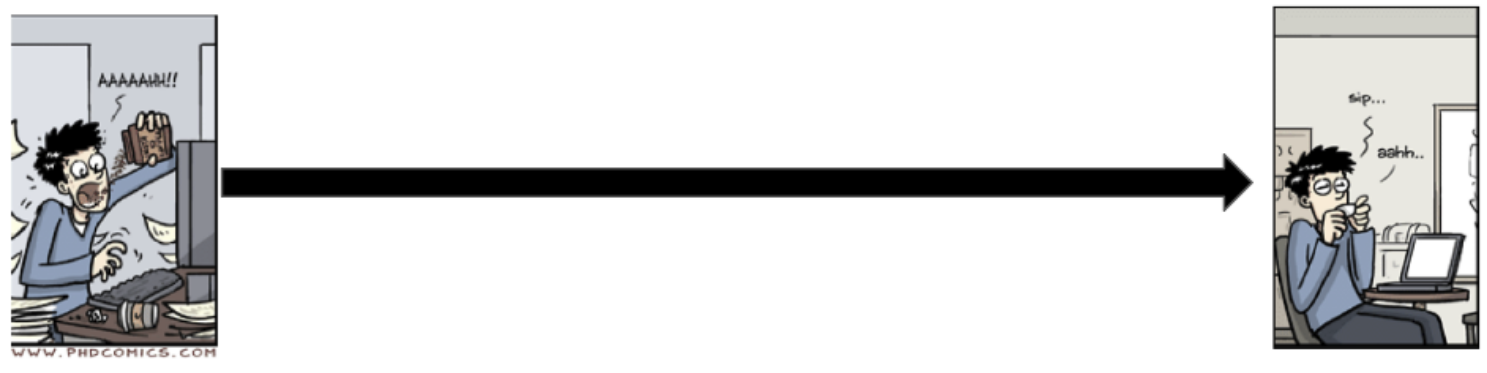
\includegraphics[scale=0.18]{../plots/motivation.png}};
	\pause
	\onslide<2> \node (img2) at (img1.south) {
\includegraphics[scale=0.18]{../plots/red_arrow.png}};
	\pause
\end{tikzpicture}
\end{center}
\begin{columns}
	\column{0.5\textwidth}
	\onslide<3-4> {2 (similar) datasets with differing size, \# of classes, class balance}		\onslide<3-4>{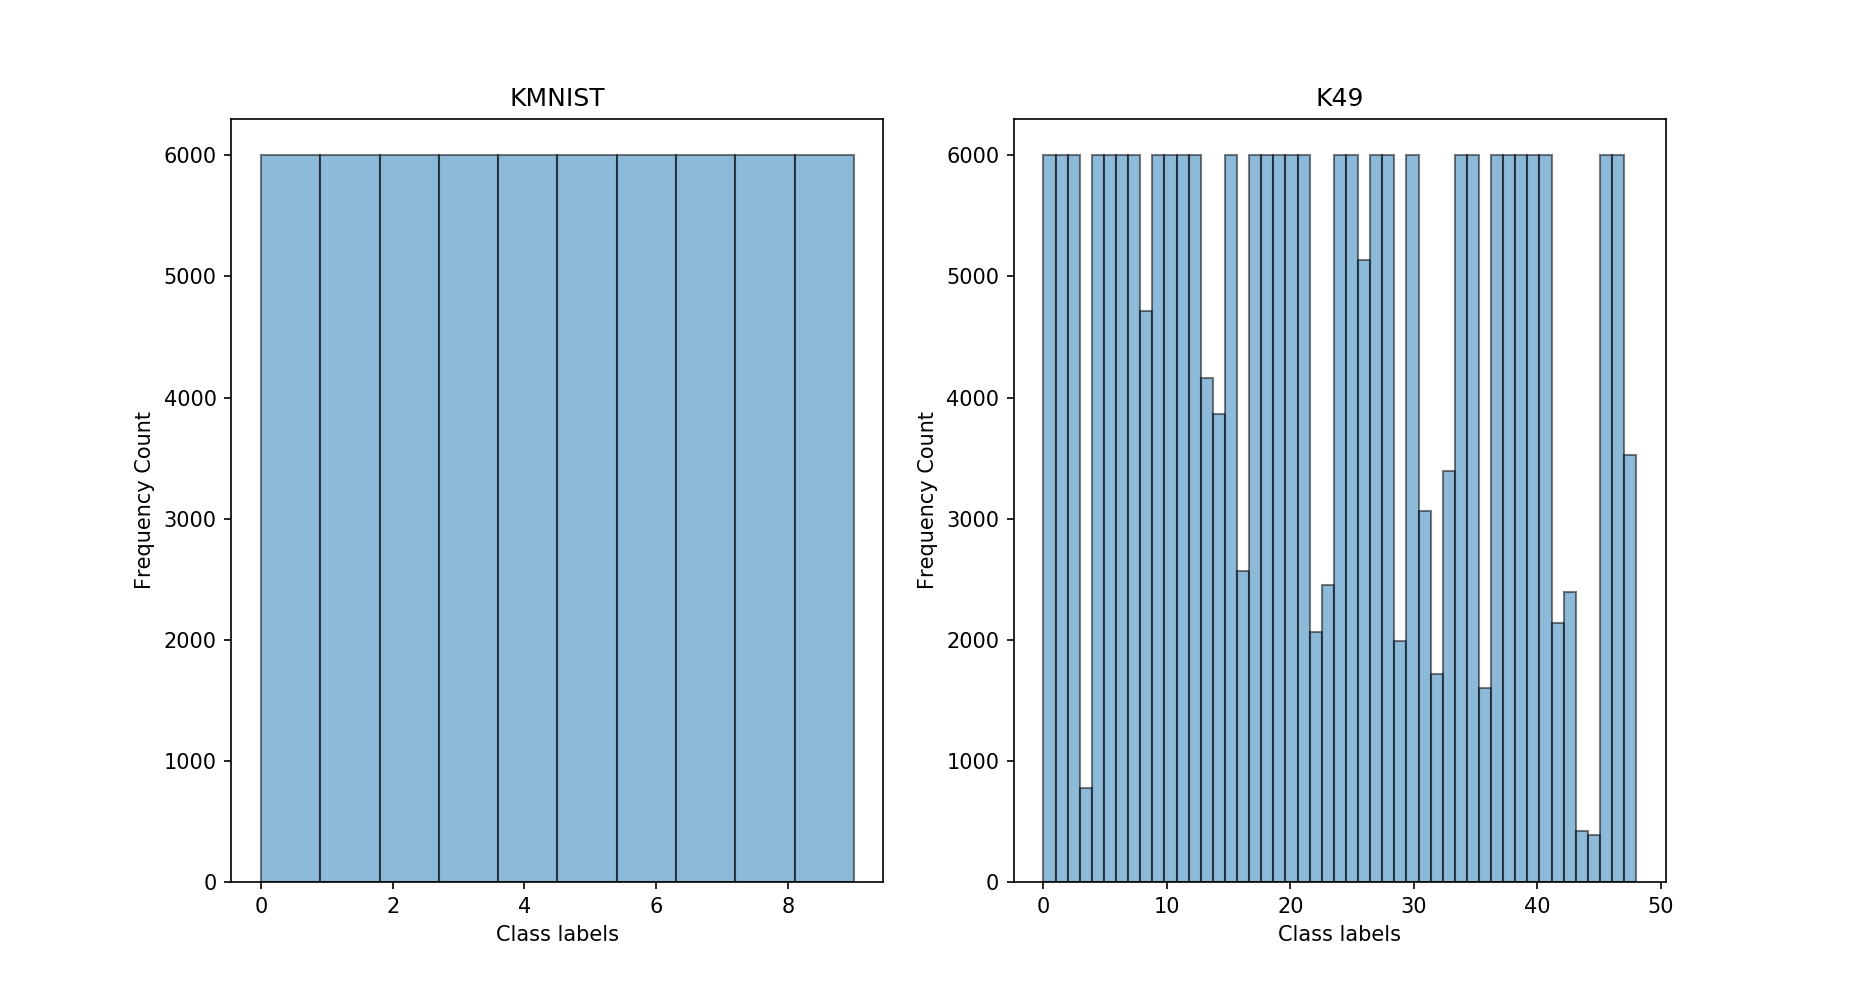
\includegraphics[width=\textwidth, height=3.5cm]{../plots/class_distro_plot.png}}
	\pause
	\column{0.5\textwidth}
	\onslide<4> {BOHB outperforms SMAC in high dimensional, mixed data}
	\onslide<4> {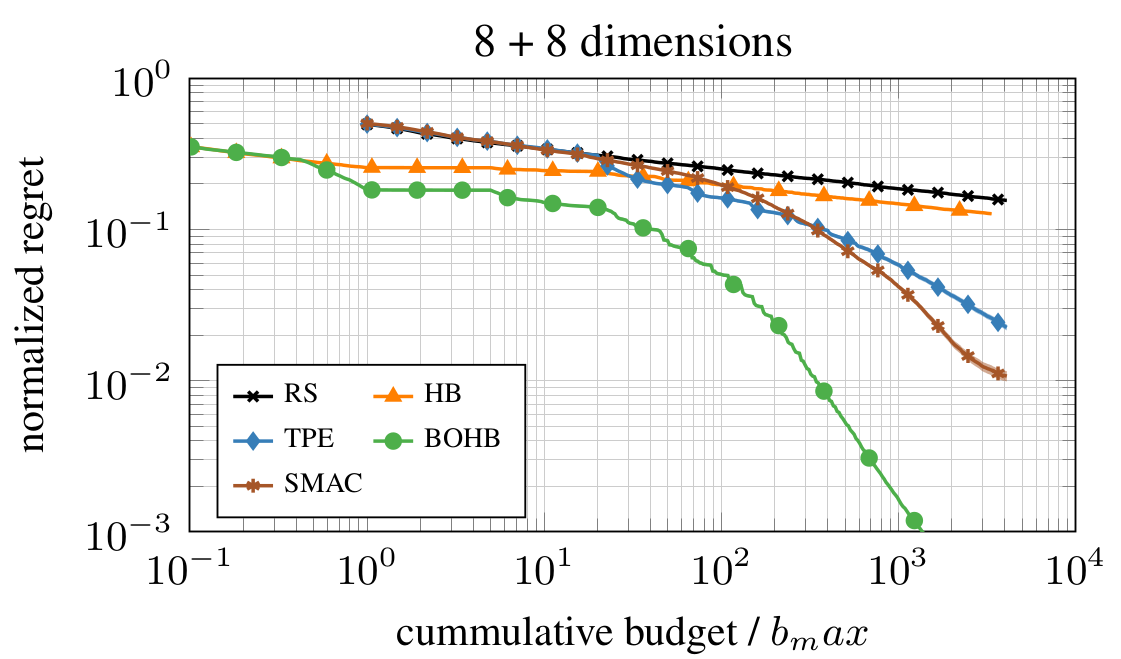
\includegraphics[width=\textwidth]{../plots/bohb_smac.png}}
\end{columns}
\end{frame}


%%
% SLIDE 2 - BOHB and SETUP
%%
\begin{frame}
\frametitle{Design Decisions (and BOHB)}
\begin{block}{CNN Structure}
 $INPUT\bm{\rightarrow}[CONV \rightarrow BATCHNORM? \rightarrow ACTIVATION \rightarrow DROPOUT? \rightarrow MAXPOOL?]*M \bm{\rightarrow} [FC \rightarrow BATCHNORM? \rightarrow ACTIVATION \rightarrow DROPOUT?]*K \bm{\rightarrow} OUTPUT$ \newline
 $ M \in \{1,2,3\}$;  $K \in \{0,1,2\}$;  $? \rightarrow \top or \bot $
\end{block}
\pause
\begin{columns}
	\column{0.5\textwidth}
	\vspace{0.3cm} 
	\begin{itemize}
		\item CONVolution layers
		\begin{itemize}
			\item Kernel size
			\item Padding
			\item Stride
		\end{itemize}
		\item ACTIVATION (relu/sigmoid/tanh)
		\item BATCHNORM, DROPOUT
		\begin{itemize}
			\item True or False
		\end{itemize}
		\item MAXPOOL (if True)
		\begin{itemize}
			\item Kernel size (=stride)
		\end{itemize}	
		\pause
		\item Learning rate
		\item Optimizer
		\item Batch size
	\end{itemize}
	\pause
	\column{0.5\textwidth}
	\begin{itemize}
		\item \textgreater 30 hyperparameters 
		\item (Budget = Epochs) $\rightarrow$ expensive runs
	\end{itemize}
%	\vspace{0.5cm} \\
	\pause
	\vspace{0.5cm} 
	\textbf{BOHB params:}
	\begin{center}
		\centering
		\begin{tabular}{c|c|c}
			eta & min\_budget & max\_budget \\
			\hline\hline
			2 & 1 & 16 \\
			4 & 1 & 16 \\
			3 & 1 & 9 \\
			2 & 1 & 10
		\end{tabular}
	\end{center}
\end{columns}
\end{frame}


%%
% SLIDE 3 - Preliminary Results
%%
\begin{frame}
\frametitle{BOHB on KMNIST (and K49)}
\begin{tabular*}{\textwidth}{|c|c|c|c|c|c|}
	\hline
	\multicolumn{1}{|p{1.5cm}|}{\centering Dataset} & 
	\multicolumn{1}{|p{2cm}|}{\centering eta\_min\_max\_iter \\ (BOHB)} & 
	\multicolumn{1}{|p{1.5cm}|}{\centering Validation \\ Accuracy} &
	\multicolumn{1}{|p{1.5cm}|}{\centering Train \\ Accuracy} &
	\multicolumn{1}{|p{1.5cm}|}{\centering Test \\ Accuracy} &
	\multicolumn{1}{|p{1.5cm}|}{\centering BOHB \\ Runtime} \\
	\hline\hline
	KMNIST & 2\_1\_16\_10 & 98.08\% & 99.81\% & 95.06\% & \textless3 hrs \\
	KMNIST & 3\_1\_9\_20 & 97.17\% & 98.23\% & 93.26\% & \textless3 hrs \\
	KMNIST & 4\_1\_16\_20 & 98.26\% & 99.98\% & 96.41\% & \textless4 hrs \\
	KMNIST & 2\_1\_10\_14 & 97.77\% & 99.86\% & 94.08\% & \textless4 hrs \\
	KMNIST & 3\_2\_20\_20 & 98.31\% & 99.62\% & 95.41\% & \textless6 hrs \\
	\hline \pause
	K49 & 3\_1\_9\_10 & 89.06\% & 99.93\% & 88.12\% & \textless5 hrs \\
	K49 & 2\_1\_10\_10 & 91.19\% & 99.25\% & 88.25\% & \textless12 hrs \\
	\hline
\end{tabular*}
\pause
\begin{figure}
	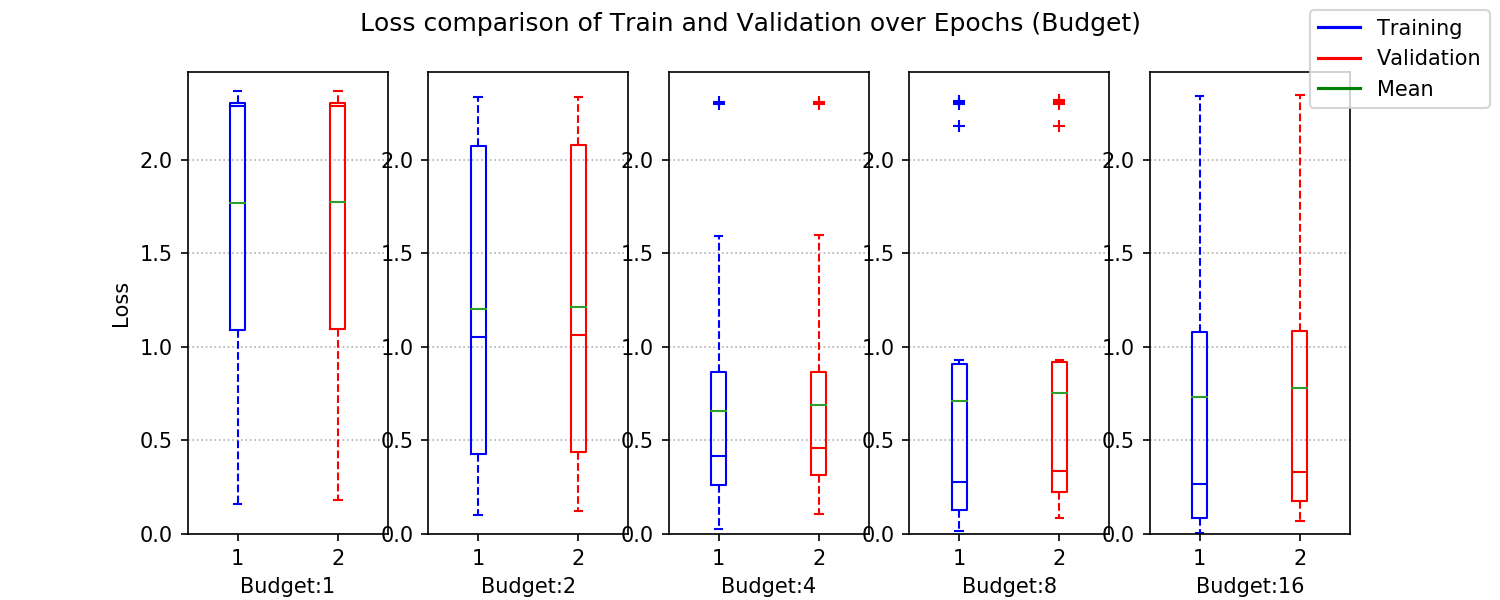
\includegraphics[width=\textwidth]{../plots/kmnist_bohb_loss_comparison_plot.png}
\end{figure}
\end{frame}


%%
% SLIDE 4 - Extracting more juice from KMNIST
%%
\begin{frame}
\frametitle{Extracting juice (Can K49 leverage KMNIST?)}
\begin{columns}
	\column{0.48\textwidth}
 	Model: KMNIST $\rightarrow$ K49 \\
	\onslide<1->\begin{tabular*}{\textwidth}{|c|c|c|c|}
%	\onslide<1->\begin{tabular*}{\textwidth}{|>{\small}c|>{\small}c|>{\small}c|>{\small}c|}
		\hline
		\multicolumn{1}{|p{1.25cm}|}{\centering KMNIST \\ Test} &
		\multicolumn{1}{|p{0.8cm}|}{\centering K49 \\ Train} &
		\multicolumn{1}{|p{0.8cm}|}{\centering K49 \\ Test} &
		\multicolumn{1}{|p{1cm}|}{\centering Run- \\ time} \\
		\hline\hline
		95.06\% & 97.15\% & 90.49\% & \textless2hrs \\
		95.41\% & 95.91\% & 90.63\% & \textless1hr \\
		96.41\% & 99.67\% & 93.32\% & \textless4hrs \\
		\hline
	\end{tabular*}
	\pause
	\vspace{0.5cm} \\
	\onslide<2->{Configuration: KMNIST $\xrightarrow{\text{BOHB}}$ K49} \\
	\vspace{0.1cm}
	\onslide<2->{Hyperparameters:
	\begin{itemize}
		\item \# of channels
		\item \# of FC layers and neurons
		\item batch size
	\end{itemize}}
	\onslide<2->\begin{tabular*}{\textwidth}{|c|c|c|c|}
%	\onslide<3->\begin{tabular*}{\textwidth}{|>{\small}c|>{\small}c|>{\small}c|>{\small}c|}
		\hline
		\multicolumn{1}{|p{1.25cm}|}{\centering KMNIST \\ Test} &
		\multicolumn{1}{|p{0.8cm}|}{\centering K49 \\ Train} &
		\multicolumn{1}{|p{0.8cm}|}{\centering K49 \\ Test} &
		\multicolumn{1}{|p{1cm}|}{\centering Run- \\ time} \\
		\hline\hline
		95.41\% & 98.87\% & 90.20\% & \textless4hrs \\
		96.41\% & 99.93\% & 94.28\% & \textless20hrs \\
		\hline
	\end{tabular*}
	\column{0.48\textwidth}
	\begin{figure}
		\onslide<2->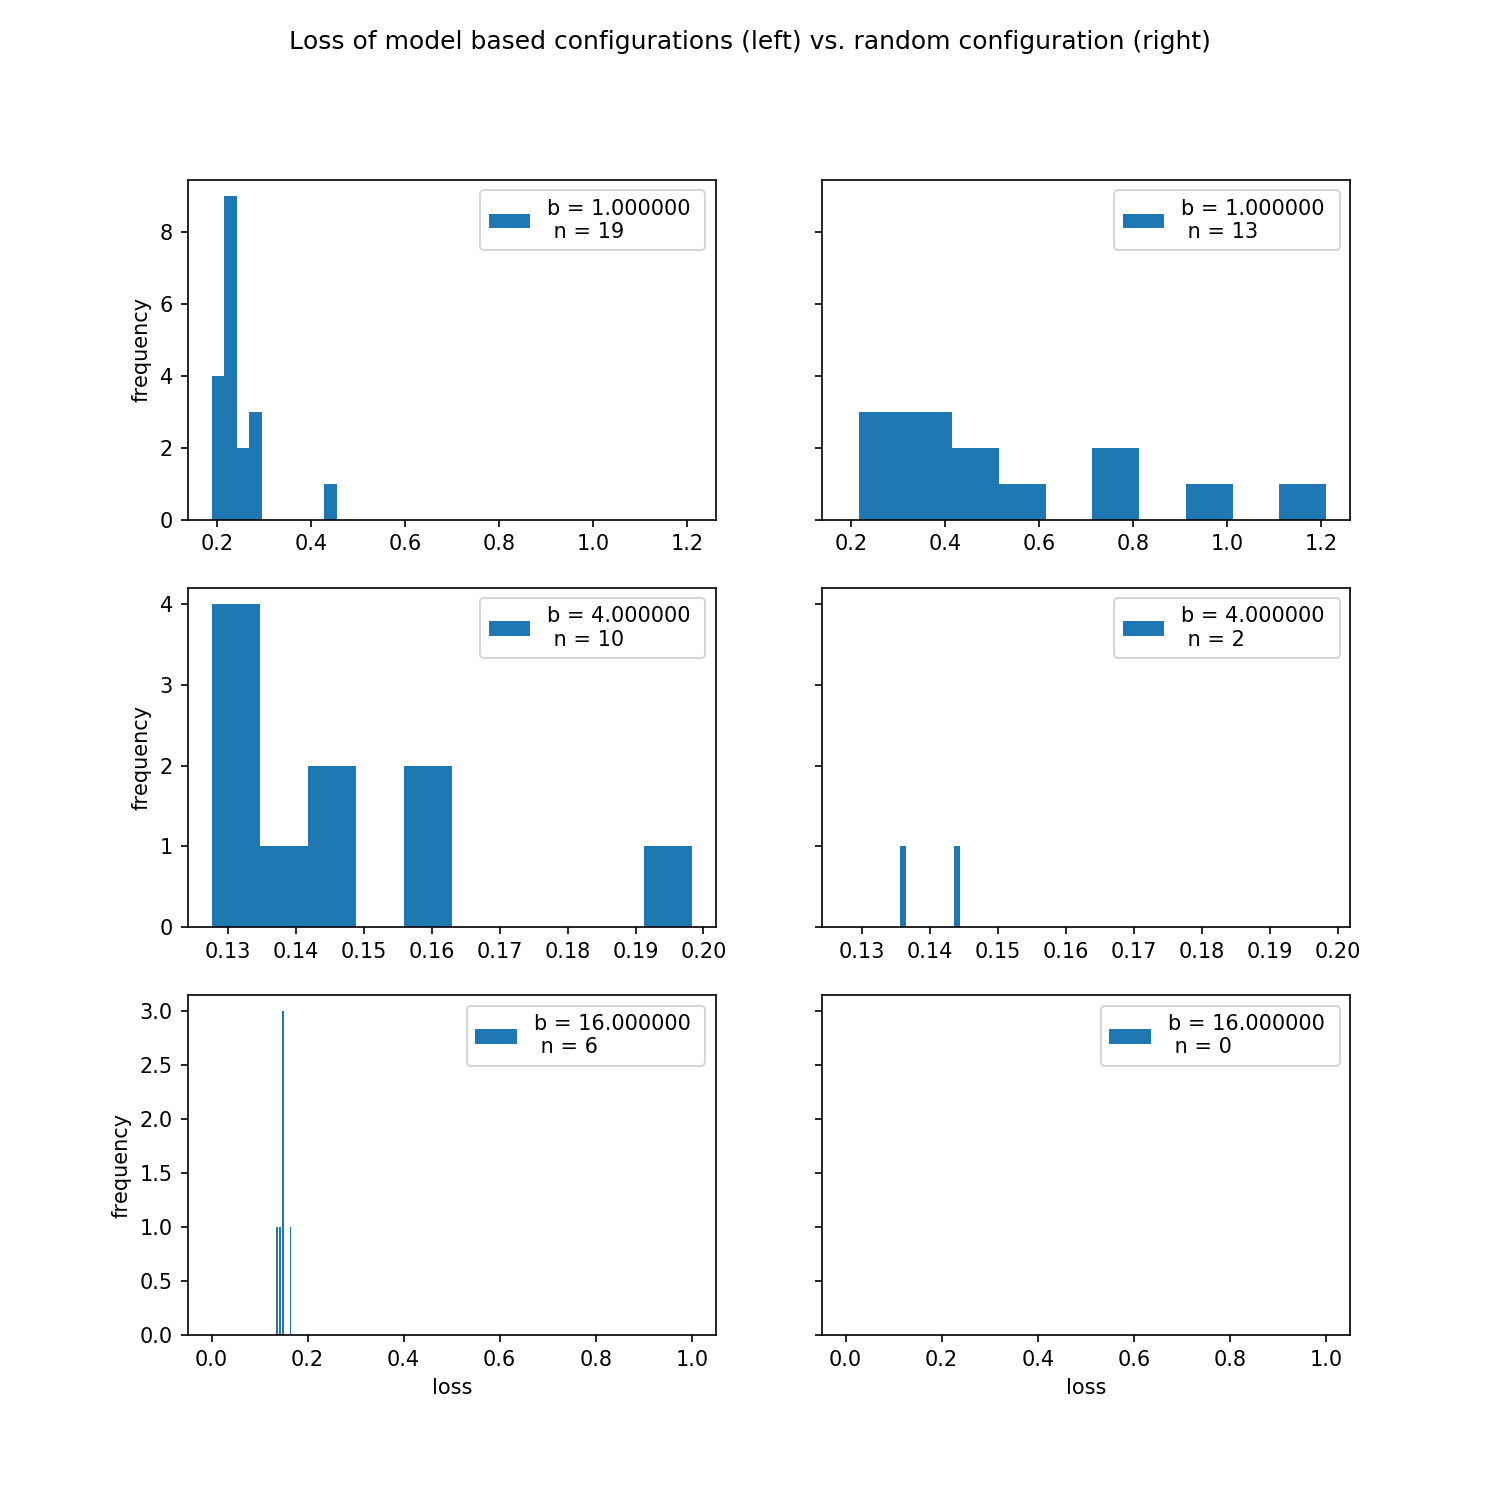
\includegraphics[height=3.1cm, width=4.5cm]{../plots/plot_performance_histogram.png}
	\end{figure}
	\onslide<3->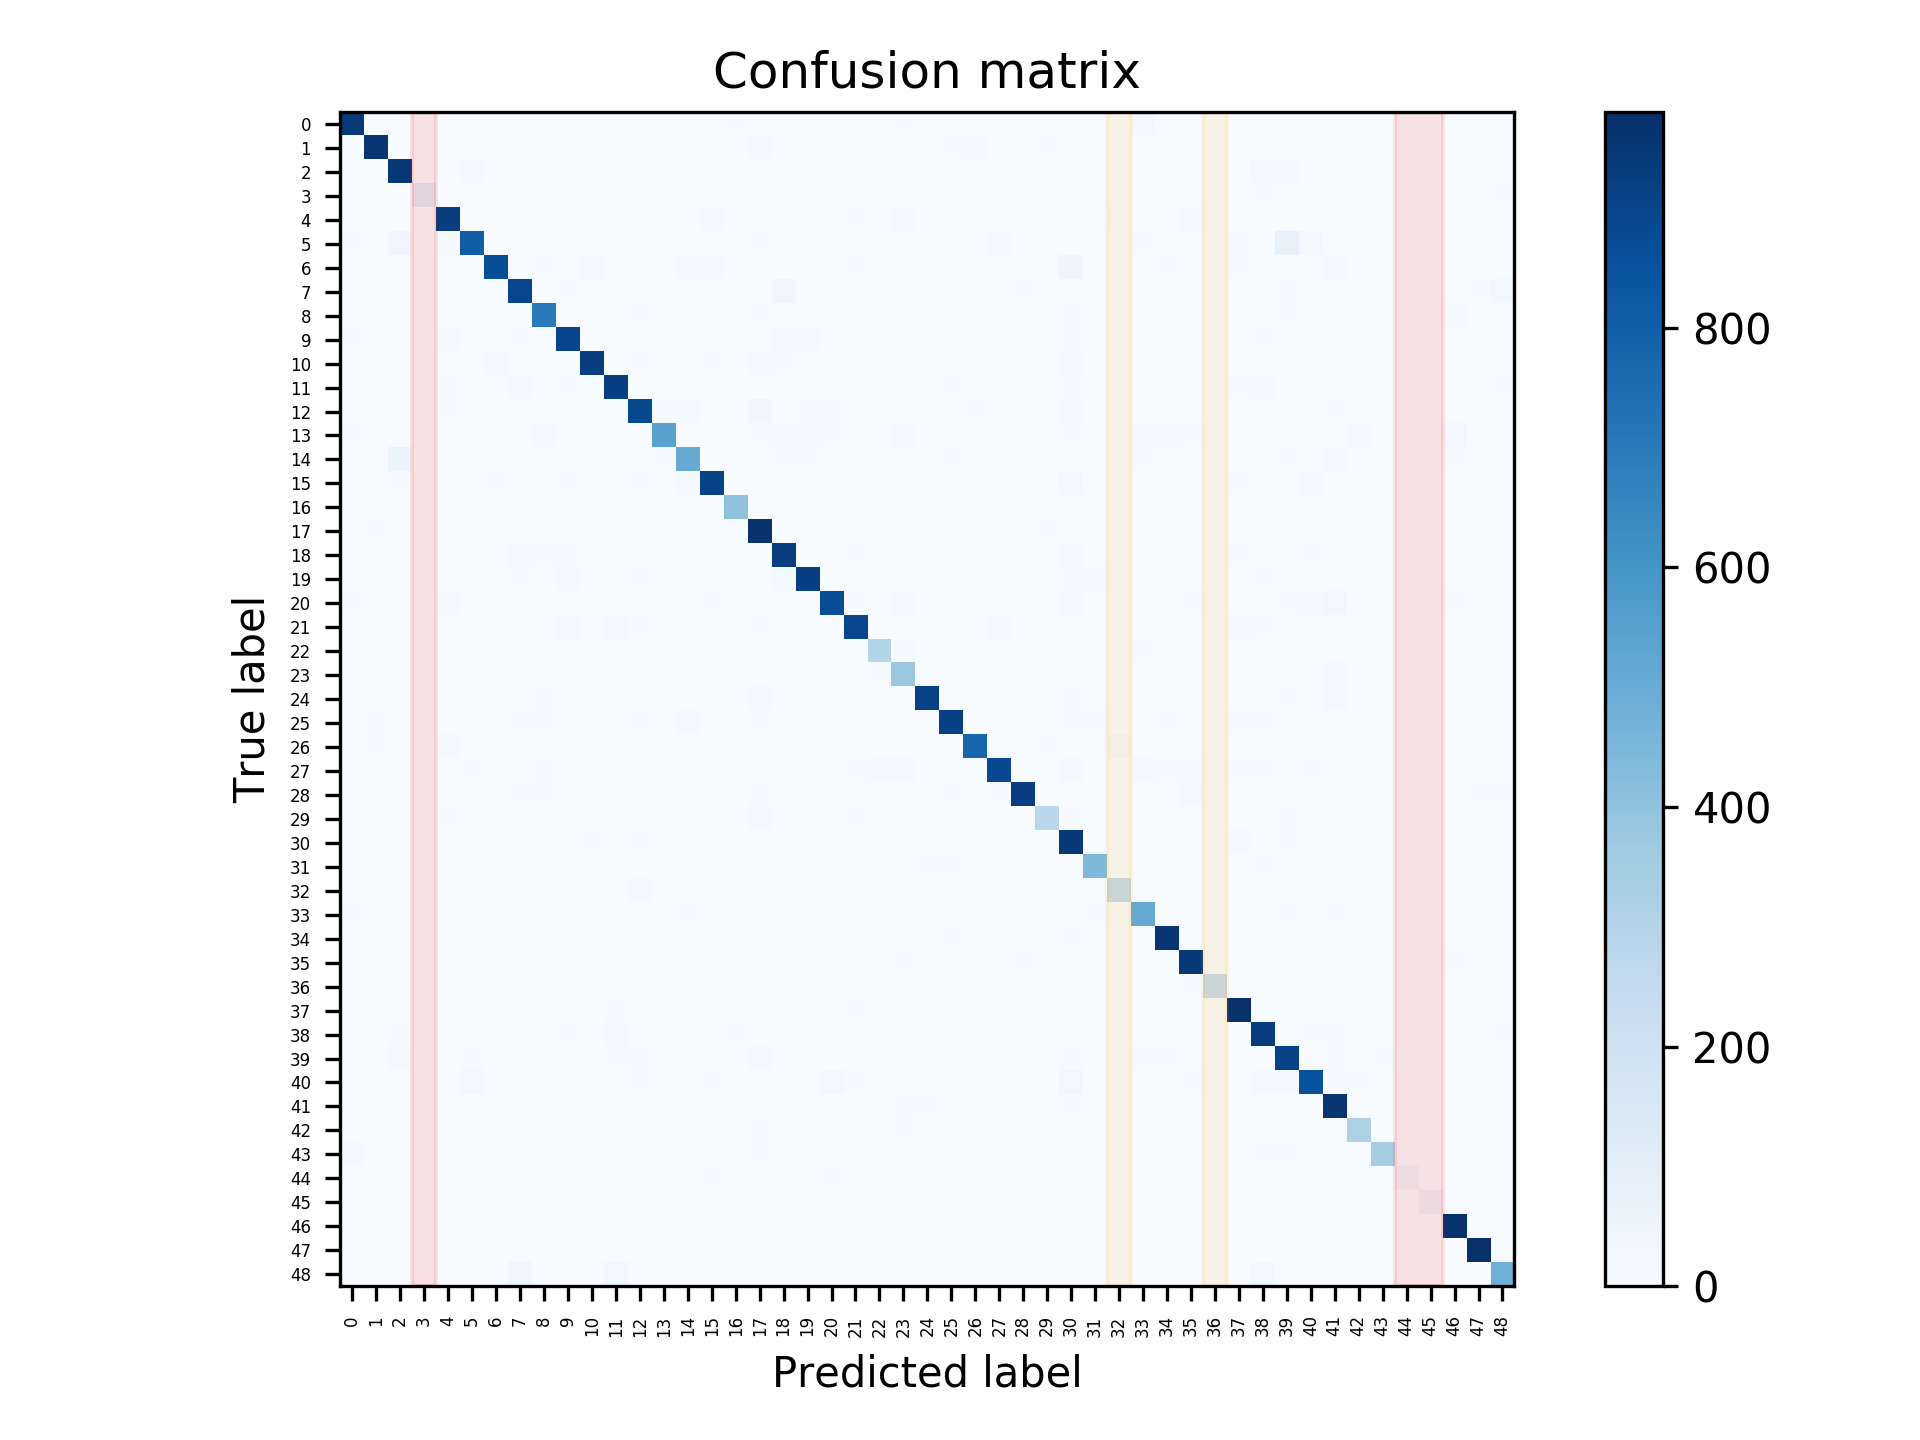
\includegraphics[height=4cm, width=\textwidth]{../plots/confusion_matrix_20.png}
\end{columns}
\pause
\vspace{0.2cm}
\onslide<3->{\underline{Issues}: (i) Under-represented classes; (ii) Slow experiments; } 
\onslide<4-> [(iii) What if only K49?]
\end{frame}


%%
% SLIDE 5 - Conclusion
%%
\begin{frame}
\frametitle{In Conclusion...}
\begin{columns}
	\column{0.5\textwidth}
	Possible improvements:
	\begin{itemize}
		\item Fidelity (data subsets)
		\begin{itemize}
			\item K49: 90.20\% $\rightarrow$ 93.85\%
		\end{itemize} 
		\pause
		\item Data Augmentation
		\begin{itemize}
			\item K49: 94.28\% $\rightarrow$ 93.37\% (with fidelity)
		\end{itemize}
		\pause
		\item Better/more parameters for transfer configuration
		\begin{itemize}
			\item Learning rate schedule
			\item Optimizer
		\end{itemize}
		\pause
		\item EPMs to try reduce parameter blow ups and runtimes
		\pause
		\item NAS cell search
		\pause
		\item Padding to go deeper (exploit sparsity)
	\end{itemize}
	\hrule
	\vspace{0.2cm}
	\underline{Final Numbers}:
	\vspace{0.15cm}
	\begin{tabular}{|c|c|c|}
		%	\onslide<3->\begin{tabular*}{\textwidth}{|>{\small}c|>{\small}c|>{\small}c|>{\small}c|}
		\hline
%		\multicolumn{1}{|p{1cm}|}{\centering Dataset} &
%		\multicolumn{1}{|p{1cm}|}{\centering Default \\ Test} &
%		\multicolumn{1}{|p{1cm}|}{\centering Best \\ Test} \\
		Dataset & Default Test & Best Test \\
		\hline\hline
		KMNIST & 69.56\% & 97.89\% \\
		\hline
		K49 & 54.43\% & 94.28\%  \\
		\hline
	\end{tabular}
	KMNIST: \textit{from transferring best K49 model}\\
	K49: \textit{from transferring incumbent config on KMNIST and then BOHB on K49}\\
	\column{0.48\textwidth}
	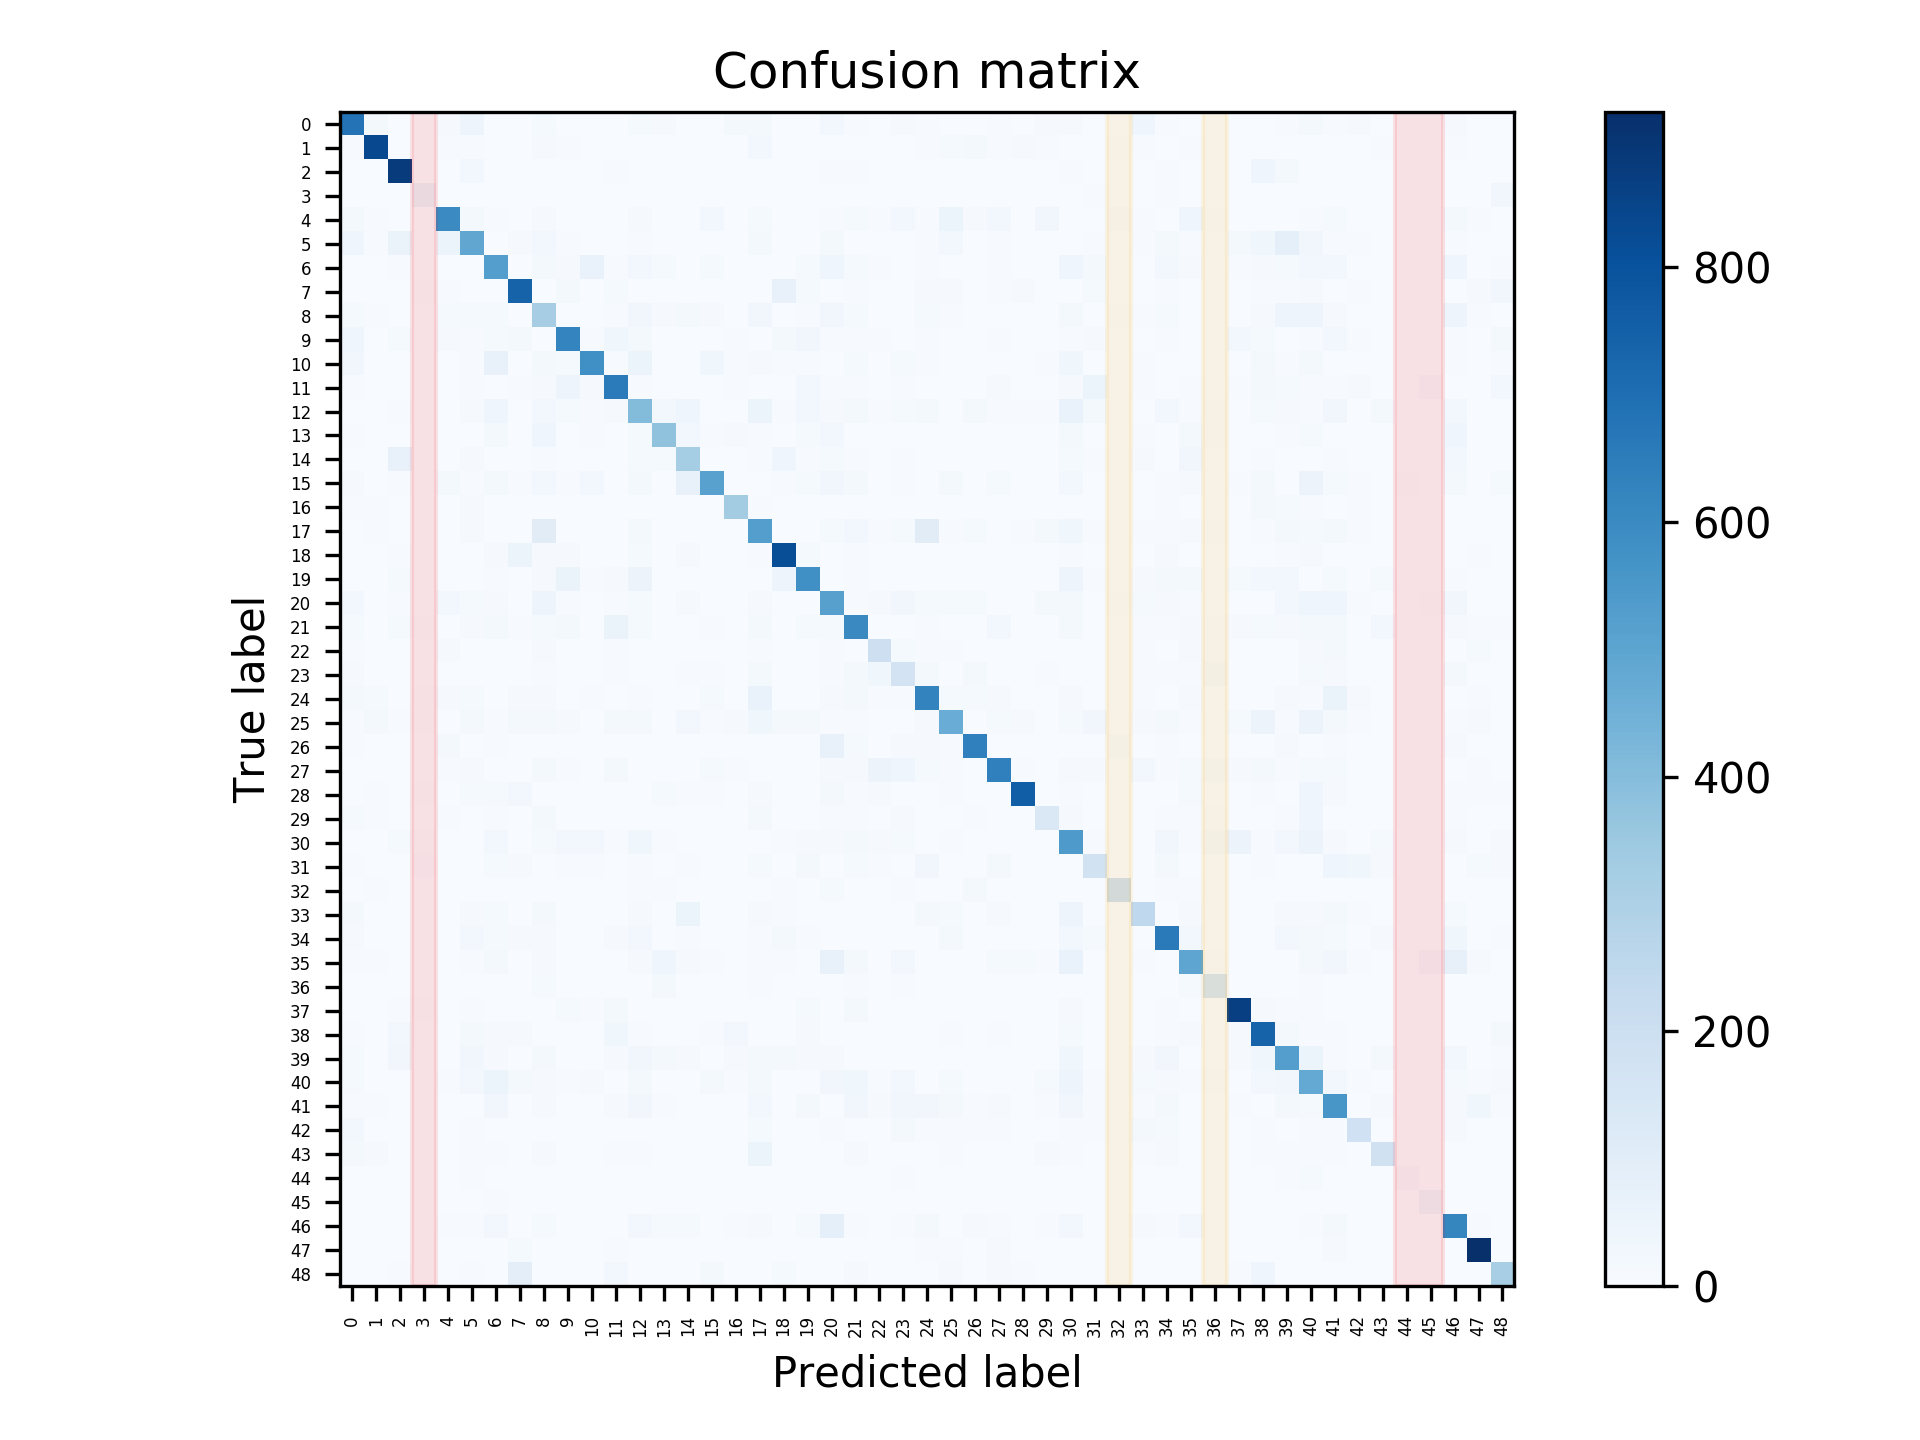
\includegraphics[height=4cm, width=6cm]{../plots/k49_confusion_matrix_default.png}
	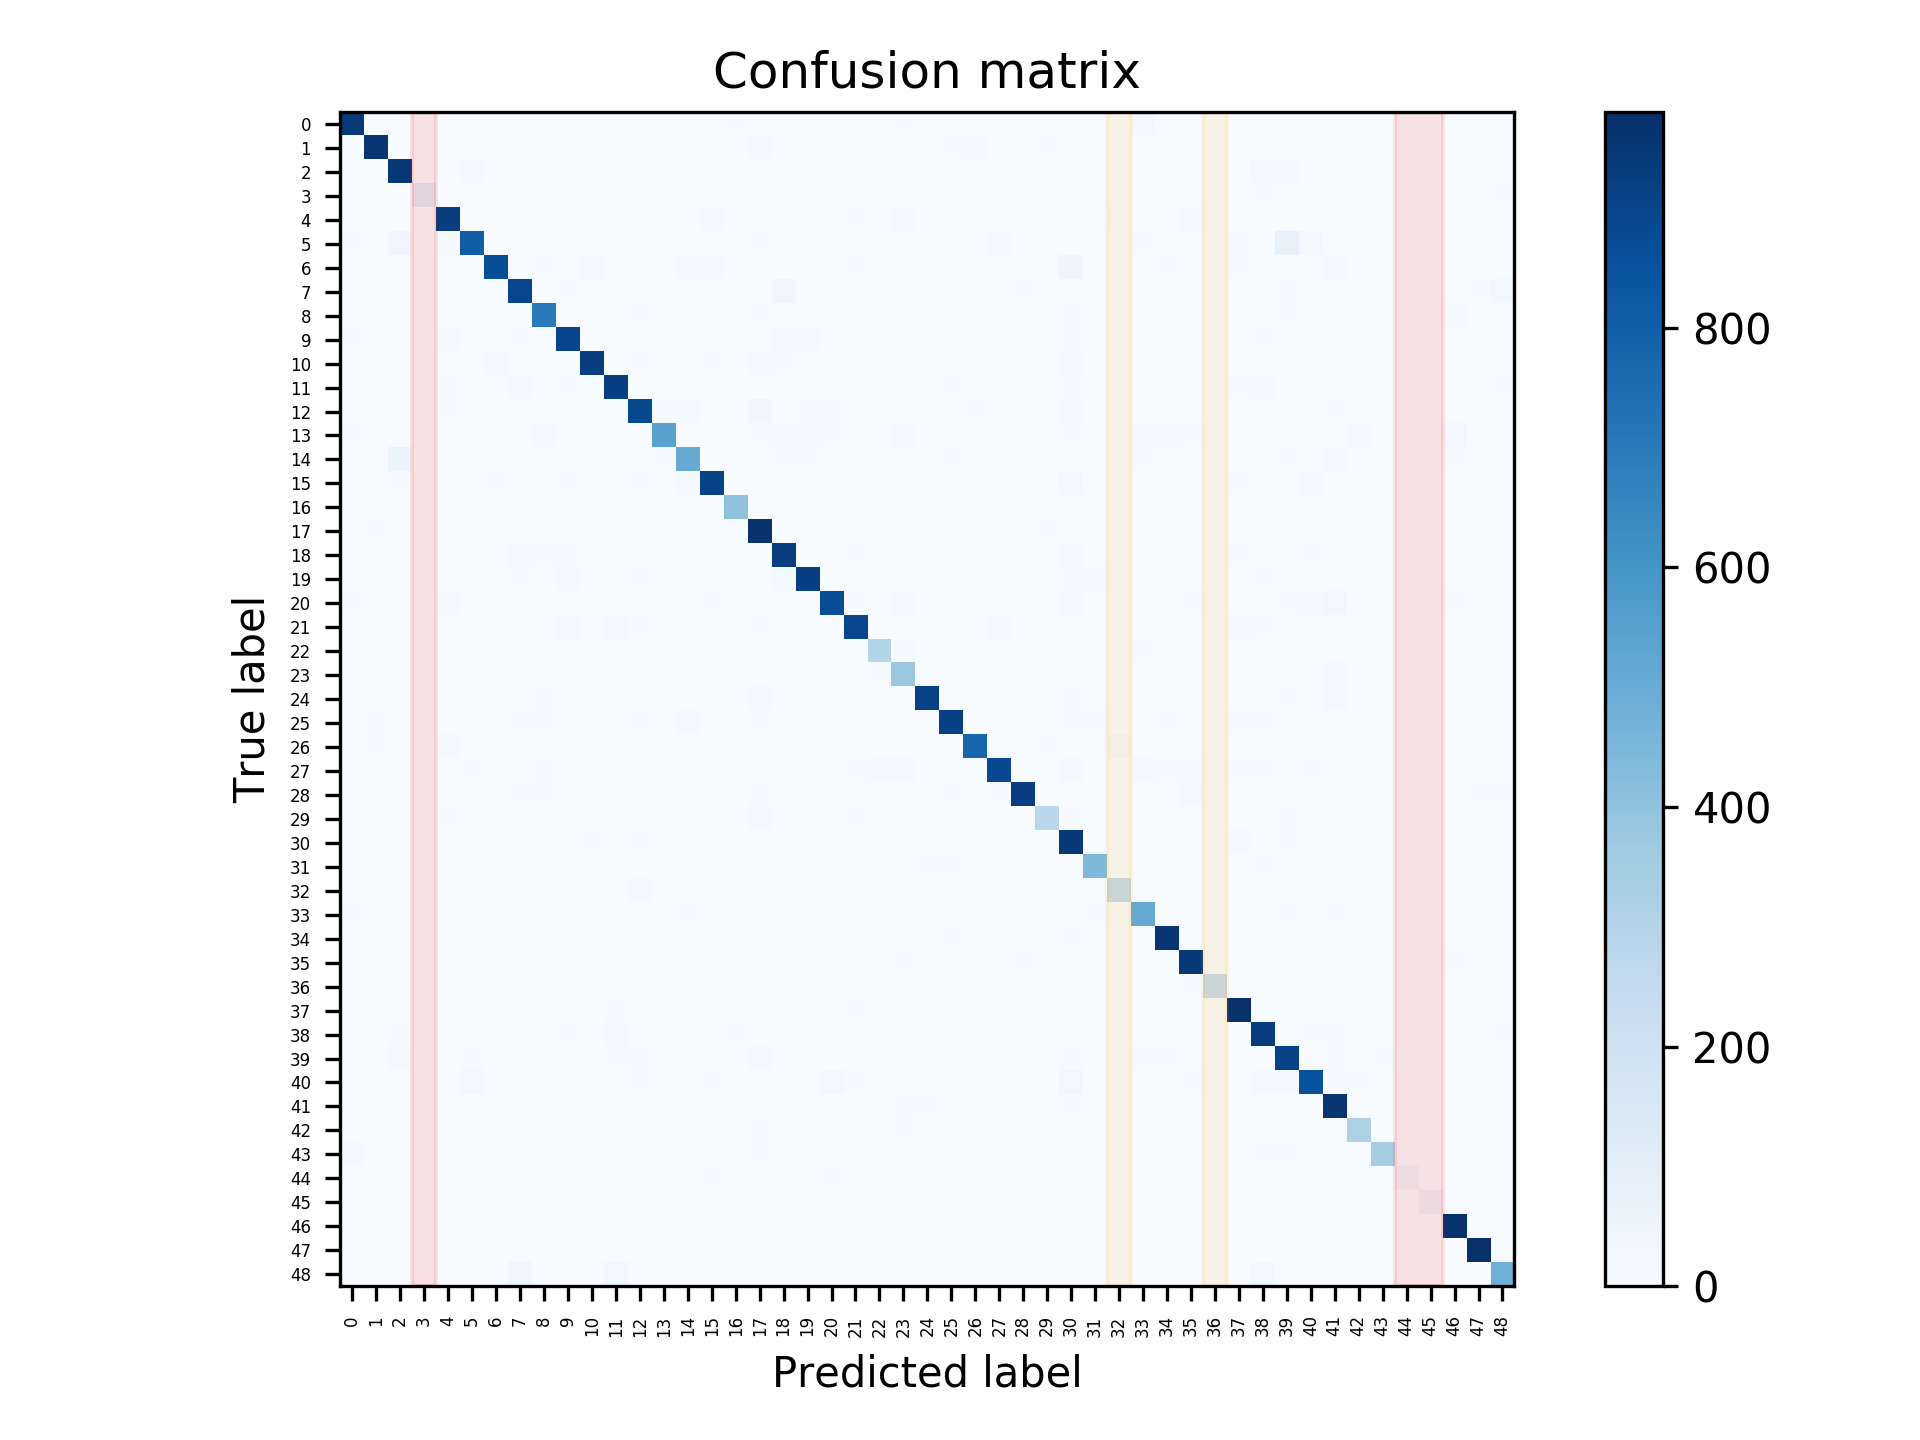
\includegraphics[height=5cm, width=7cm]{../plots/confusion_matrix_20.png}
\end{columns}\end{frame}

%\begin{onlyenv}<3-6>
%	\begin{center}
%		\includegraphics<3>[scale=0.4]{image-a}
%		\includegraphics<4>[scale=0.4]{image-b}
%		\includegraphics<6>[scale=0.4]{image-c}
%	\end{center}
%\end{onlyenv}

\end{document}